% Copyright (C) Data Structures and Algorithms Team.
\chapter{Heap}
A heap can be thought of as a simple tree data structure, however a heap usually employs one of two strategies:

\begin{enumerate}
\item min heap; or
\item max heap
\end{enumerate}

Each strategy determines the properties of the tree and it's values, e.g. if you were to choose the strategy min heap then each parent node would have a value that is $\leq$ than it's children, thus the node at the root of the tree will have the smallest value in the tree, the opposite is true if you were to use max heap. Generally as a rule you should always assume that a heap employs the min heap strategy unless otherwise stated.

Unlike other tree data structures like the one defined in \S\ref{bst} a heap is generally implemented as an array rather than a series of nodes who each have references to other nodes, both however contain nodes that have at most two children. Figure \ref{fig:tree_array_representation} shows how the tree (not a heap data structure) ($12~7$($3~2$)~$6$($9$~~)) would be represented as an array.

\begin{figure}
\begin{center}
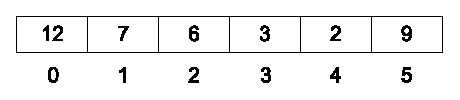
\includegraphics{heap_tree_array_representation}
\end{center}
\caption{Array representation of a simple tree data structure} \label{fig:tree_array_representation}
\end{figure}

Because we are using an array we need some way to calculate the index of a parent node, and the children of a node this is very simple, the expressions are defined below:

\begin{enumerate}
\item ($index - 1$)/$2$ (parent index)
\item $2 * index + 1$ (left child)
\item $2 * index + 2$ (right child)
\end{enumerate}

In Figure \ref{fig:heap_tree_array_representation_indexes} a) represents the calculation of the right child of $12$ ($2 * 0 + 2$); and b) calculates the index of the parent of $3$ (($3 - 1$)/$2$).

\begin{figure}
\begin{center}
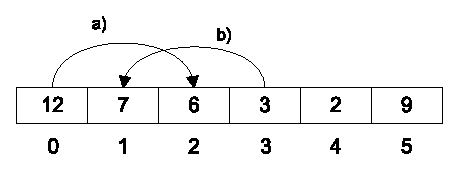
\includegraphics{heap_tree_array_representation_indexes}
\caption{Calculating node properties} \label{fig:heap_tree_array_representation_indexes}
\end{center}
\end{figure}

\section{Insertion}
Adding an item to a heap has an $O(log~n)$ run time complexity, this is due to the fact that after every insertion we must verify that the heap ordering strategy used is preserved, if not we must swap the values appropriately as we work up through the sub tree's starting with the sub tree the last value was added to.


Designing an algorithm for heap insertion is simple, however we must ensure that heap order is preserved after each insertion - generally this is a post insertion operation. Inserting a value into the next free slot in an array is simple, we just need to keep track of, and increment a counter after each insertion that tells us the next free index in the array. Inserting our value into the heap is the first part of the algorithm, the second is validating heap order which in the case of min heap ordering requires us to swap the values of a parent and it's child if the value of the child is $<$ the value of it's parent, we must do this for each sub tree the value we just inserted is a constituent of.

Figure \ref{fig:heap_insertion_minify_steps} shows the steps of inserting the values $3$, $9$, $12$, $7$, and $1$ into a min heap.

\begin{figure}
\begin{center}
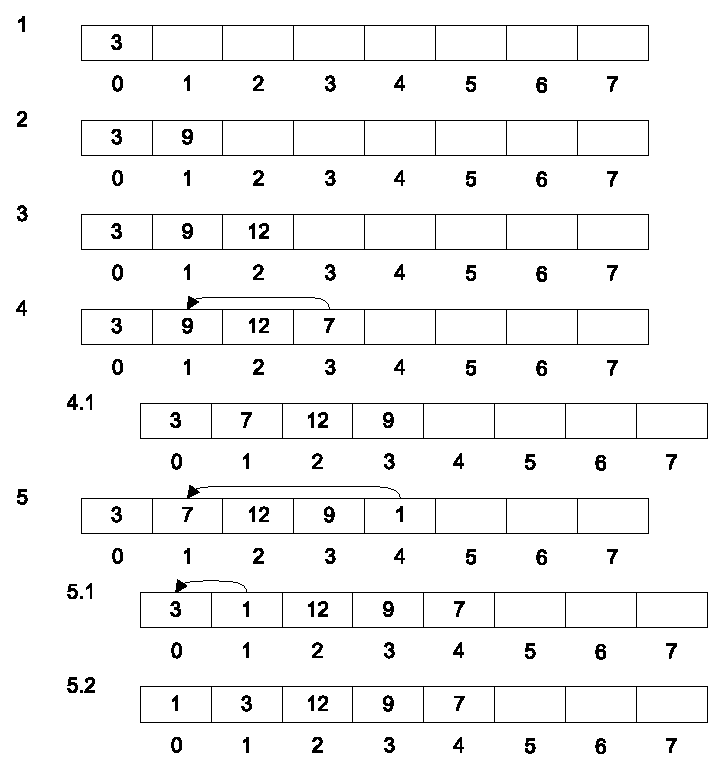
\includegraphics{heap_insertion_minify_steps}
\end{center}
\caption{Inserting values into a min heap} \label{fig:heap_insertion_minify_steps}
\end{figure}

\begin{tabbing}
1)  \textbf{alg}\= \textbf{orithm} Add($value$) \\
2)  \> \textbf{Pre:}~~$value$ is the value to add to the heap \\
3)  \> ~~~~~~~~Count is the number of items in the heap \\
4)  \> \textbf{Post:}~the value has been added to the heap \\
5)  \> $heap$[Count] $\leftarrow value$ \\
6)  \> Count $\leftarrow$ Count $+ 1$ \\
7)  \> MinHeapify() \\
8)  \textbf{end} Add \\
\end{tabbing}

\begin{tabbing}
1)  \textbf{alg}\= \textbf{orithm} MinHeapify() \\
2)  \> \textbf{Pre:}~~Count is the number of items in the heap \\
3)  \> ~~~~~~~~$heap$ is the array used to store the heap items \\
4)  \> \textbf{Post:}~the heap has preserved min heap ordering \\
5)  \> $i \leftarrow$ Count $- 1$ \\
6)  \> \textbf{whi}\= \textbf{le} $i >0$ \textbf{and} $heap$[$i$] $< heap$[($i - 1$)/$2$] \\
7)  \> \> Swap($heap$[$i$], $heap$[($i - 1$)/$2$] \\
8)  \> \> $i \leftarrow$ ($i - 1$)/$2$ \\
9)  \> \textbf{end while} \\
10) \textbf{end} MinHeapify \\
\end{tabbing}
